% Quorum, AC215 Milestone 1 statement of work. PDF to Canvas by 9:00 PM, 29 Sep.
% Dev docket numbers measured against the Regulations.gov API, 20 and 27 Sep 2026.

\documentclass[11pt]{article}

\usepackage[T1]{fontenc}
\usepackage[utf8]{inputenc}
\usepackage[margin=0.9in]{geometry}
\usepackage{microtype}
\usepackage{booktabs}
\usepackage{array}
\usepackage{graphicx}
\usepackage{enumitem}
\usepackage{xcolor}
\usepackage[colorlinks=true,allcolors=blue!60!black]{hyperref}
\usepackage{titlesec}

\titleformat{\section}{\large\bfseries}{\thesection}{0.6em}{}
\titlespacing*{\section}{0pt}{10pt}{4pt}
\setlength{\parskip}{5pt}
\setlength{\parindent}{0pt}
\setlist{itemsep=1pt, topsep=2pt, parsep=0pt, leftmargin=1.2em}
\newcolumntype{L}[1]{>{\raggedright\arraybackslash}p{#1}}

\begin{document}

\begin{center}
{\LARGE\bfseries Quorum}\\[3pt]
{\large Who is behind a public comment campaign?}\\[6pt]
\small
Aidan Eichman (aidaneichman@g.harvard.edu) \textperiodcentered{}
Aadil Jamari (ajamari@g.harvard.edu)\\
Livia Jonnatan (liviajonnatan@g.harvard.edu) \textperiodcentered{}
Andrew Yuan (ayuan@g.harvard.edu)\\
Rishi Jain (rishi\_jain@brown.edu)
\end{center}

\section{Background and motivation}

Before changing a regulation, a federal agency must take public comments and respond to them. Big
rules draw hundreds of thousands, mostly form letters. A letter sent by 40{,}000 members of an
advocacy group is legitimate. The same letter filed under 40{,}000 stolen names is fraud, and the
two look identical when they arrive.

This is not hypothetical. In the FCC's 2017 net neutrality docket, about 18 million of 22 million
comments were fake, which the New York Attorney General established four years later by subpoena
[4]. Kao had found the largest fake cluster from public data in 2017: 1.3 million comments with
synonyms swapped in so that no two matched [2].

Agencies already group form letters. On our development docket, EPA's 2019 ``waters of the United
States'' rule, staff filed 507{,}230 comments under 201 campaign records, and 92 of them list the
sponsor as unknown. Grouping is largely solved (F1 around 0.98 [1]). Nothing tells an analyst who is
behind a campaign or whether its senders are real.

\textbf{Stakeholders:} agency staff who have to answer the record; journalists, inspectors general
and attorneys general who audit it; and advocacy groups, whose real members get discounted whenever
fraud comes to light. The project grew out of reading Kao's analysis and the NY AG report.

\section{Problem statement}

Given a rulemaking docket, find its comment campaigns and show, for each one, its size, timing,
arguments, and the evidence on whether real people sent it, without labelling any individual
comment as fake.

\section{Data sources}

\begin{center}
\small
\renewcommand{\arraystretch}{1.25}
\begin{tabular}{@{}L{0.22\textwidth}L{0.55\textwidth}L{0.17\textwidth}@{}}
\toprule
\textbf{Source} & \textbf{Contents} & \textbf{Use} \\
\midrule
Regulations.gov API & Docket \texttt{EPA-HQ-OW-2018-0149}: 11{,}444 records, including 201 campaign
records (507{,}230 comments) whose PDFs list each signer's name, city and ZIP & development \\
FCC ECFS API & Docket 17-108: 23{,}982{,}072 filings with filer name and address & validation \\
NY AG report [4]; Weiss [3] & Which FCC campaigns were fake; 1{,}001 machine-written comments & labels \\
Federal Register API & Text of each proposed rule & provisions \\
\bottomrule
\end{tabular}
\end{center}

\textbf{Key attributes.} Comment text, receipt date, campaign copy count and sponsor, and signer
name, city and ZIP. ECFS adds filer name, address and timestamp.

\textbf{Relevance.} EPA's campaign records give us grouping labels for free. Signer details let us
check each campaign for signs of fake senders. The FCC docket is the only one where fraud was proven,
so that is where we validate.

\textbf{Data quality.}
\begin{itemize}
  \item Each comment body needs its own API call, 11.4 hours per key for the dev docket. We split it
        across five keys and version the result.
  \item 106 of the 201 campaigns attach only a sample letter. We keep their counts but cannot check
        their senders.
  \item Receipt dates have no time of day, so arrival is measured per day.
  \item Individual comments rarely carry a name (1 of 25 sampled), so sender checks run per campaign.
  \item All 13 campaign PDFs we sampled have a text layer. We OCR only the ones that do not.
\end{itemize}

\section{Scope and preliminary design}

\textbf{Scope.} One Regulations.gov docket end to end, with the FCC docket for validation only. We are
not building a fraud classifier, and no person gets a score.

\textbf{Pipeline.} \emph{Ingest} comments and PDFs into one record per comment. \emph{Group} them with
MinHash, using embeddings and HDBSCAN only for what MinHash misses. \emph{Characterize} each campaign
by size, daily arrival, how its copies vary, and sender checks such as a city that does not match its
ZIP. \emph{Locate} the rule provisions it argues about by retrieval over the rule text. Each step has
to beat a simpler baseline:

\begin{center}
\small
\renewcommand{\arraystretch}{1.25}
\begin{tabular}{@{}L{0.14\textwidth}L{0.2\textwidth}L{0.38\textwidth}L{0.2\textwidth}@{}}
\toprule
\textbf{Step} & \textbf{Baseline} & \textbf{Test data} & \textbf{Metric} \\
\midrule
Group & exact match; MinHash alone & EPA's 201 campaigns; 300 labelled pairs; a letter paraphrased at
5 strengths & pairwise F1 \\
Characterize & text only & NY AG campaigns; Weiss's comments; Kao's cluster & recall@$k$ \\
Locate & keyword search & 50 hand-mapped campaigns & top-1 accuracy \\
\bottomrule
\end{tabular}
\end{center}

\textbf{Success.} Reproduce EPA's groupings at pairwise F1 of 0.95 or better, and rank the NY AG's
fake campaigns above genuine ones. If timing and sender checks add nothing over text alone, we report
that. For an analyst, success means seeing every campaign and its evidence on one screen instead of
keyword search.

\textbf{Components.} Large, heterogeneous data (half a million letters, two APIs, text and PDF) and
scalability (24 million FCC filings, processed as a stream).

\textbf{Learning emphasis.} Locality-sensitive hashing, density clustering, RAG with a vector
database, and evaluation without ground truth. We use an off-the-shelf embedding model and
Tesseract, and build the rest.

\noindent\begin{minipage}{\textwidth}
\textbf{Application mock.}\\[4pt]
\centering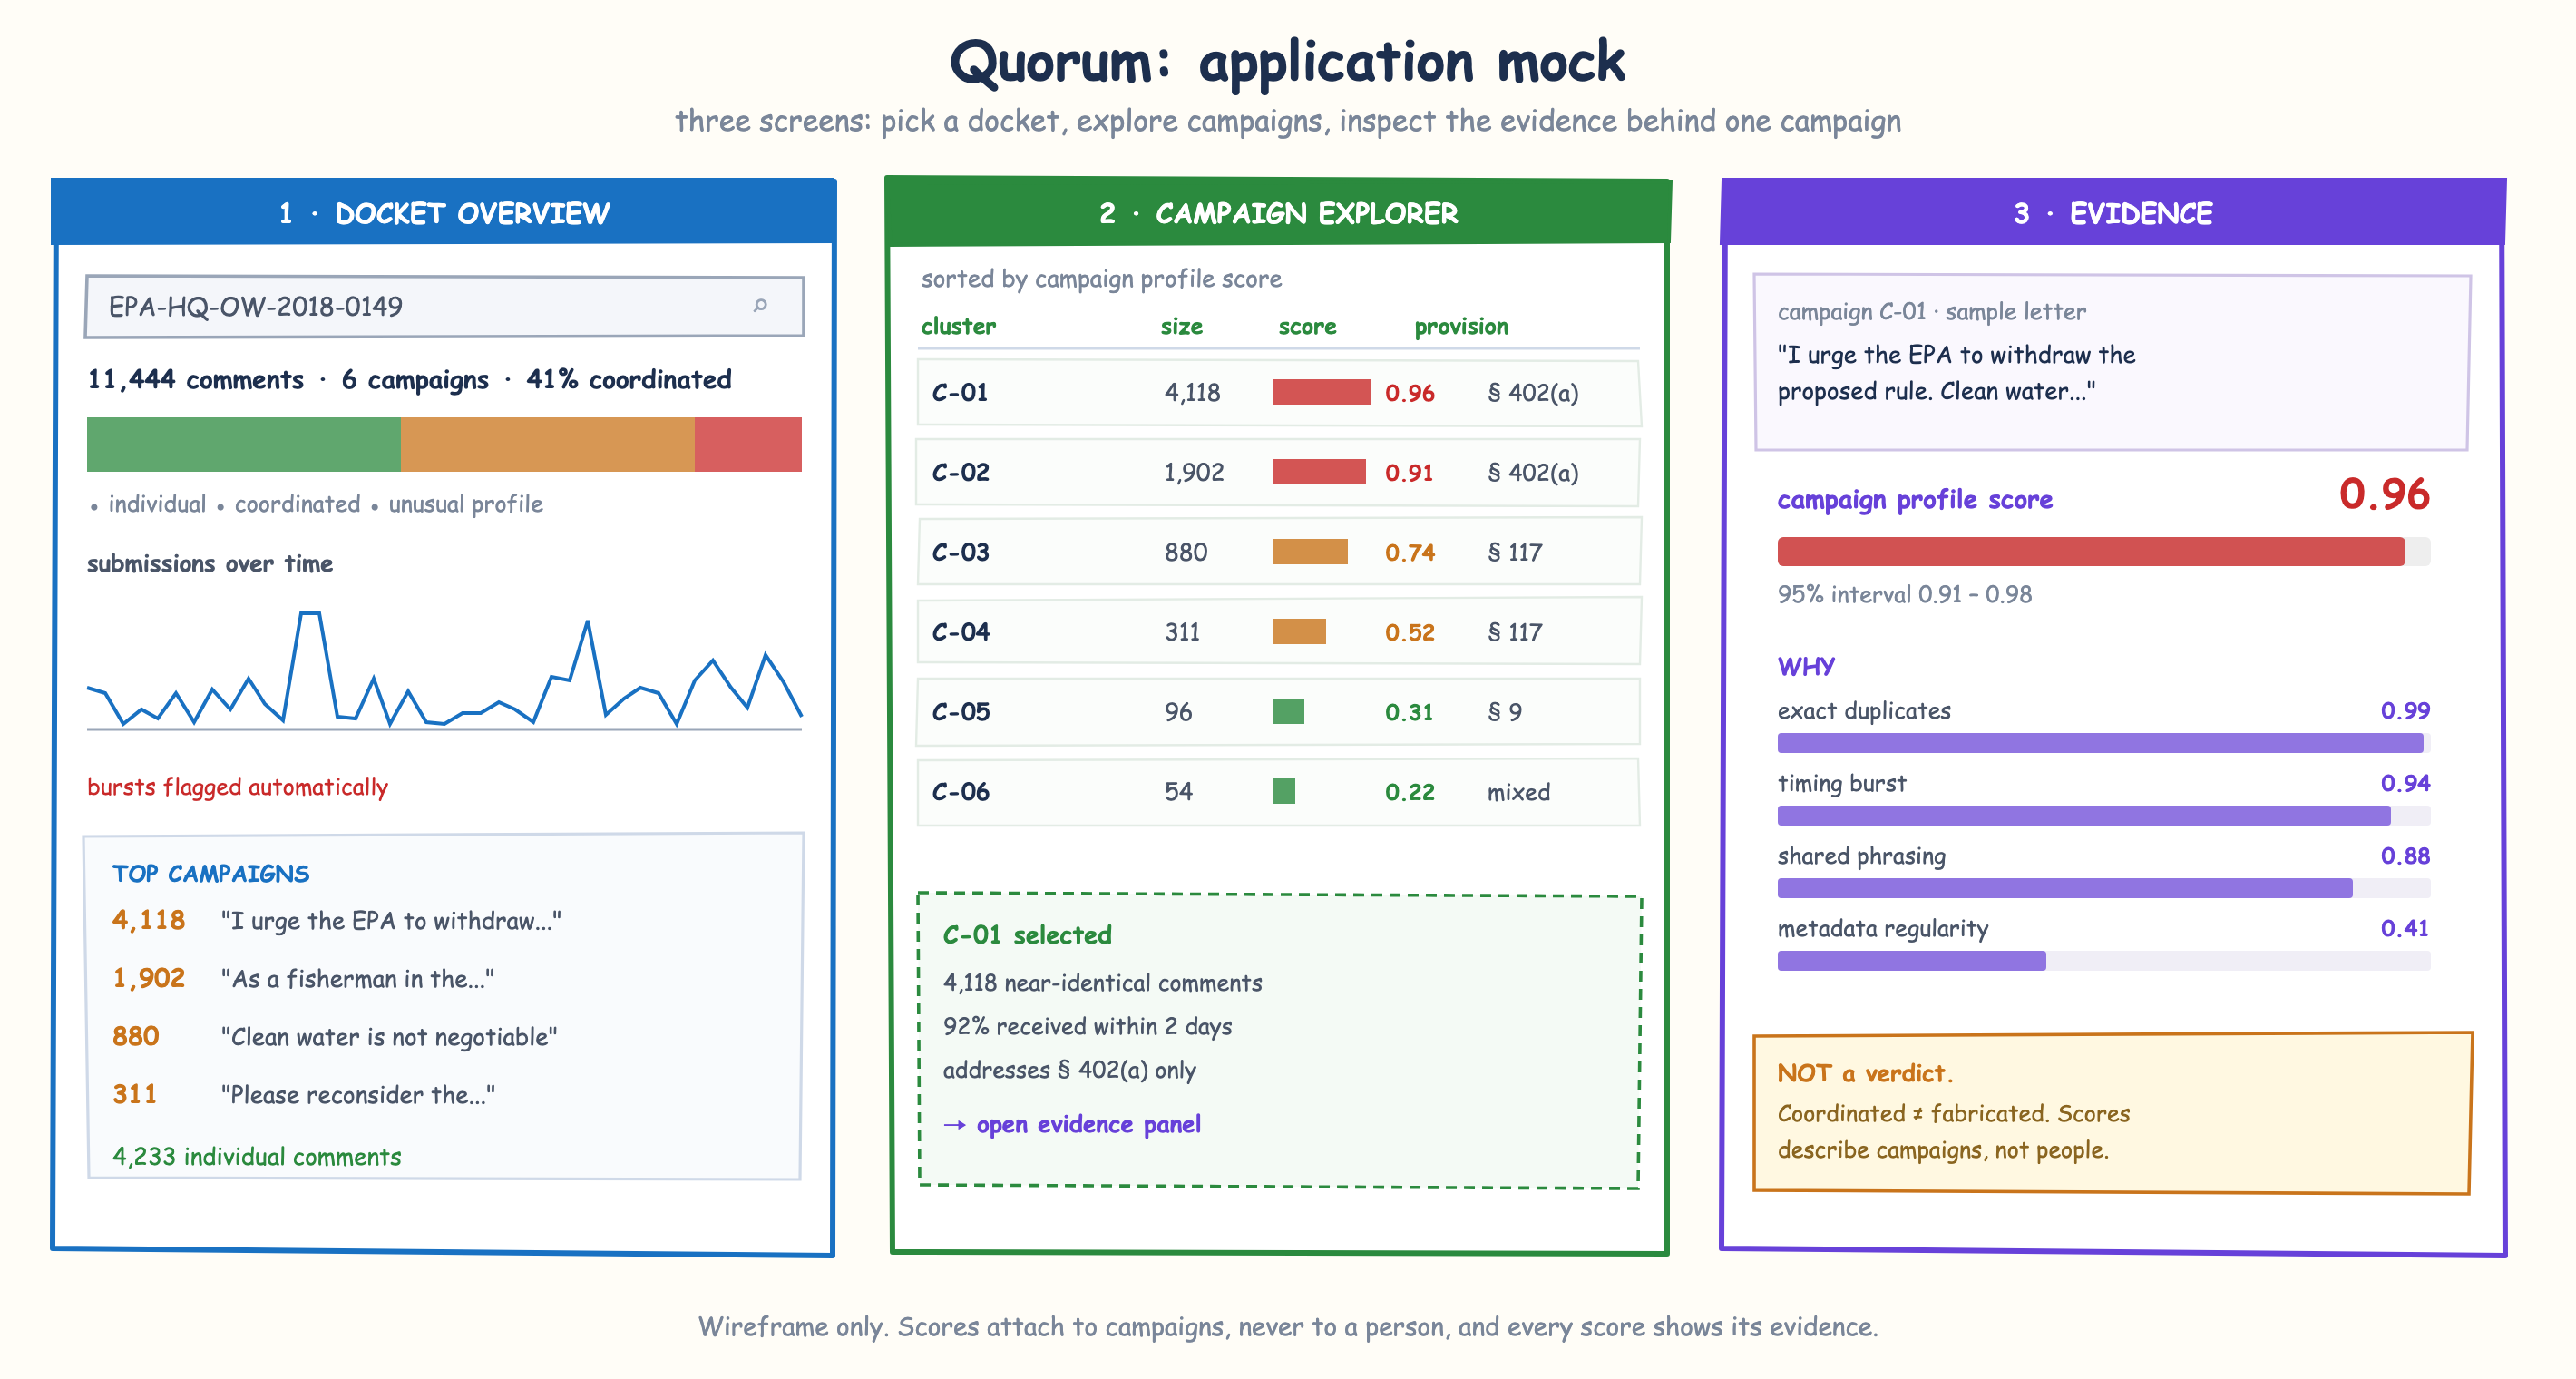
\includegraphics[width=0.8\textwidth]{docs/mock.png}
\end{minipage}

\textbf{Fun factor.} EPA lists no sponsor for 92 of the campaigns on our docket. We want to find out who sent them.

\textbf{Limitations and risks.} The worst error is making a genuine campaign look fraudulent, so
scores describe campaigns and always show their evidence. The FCC labels cover only a few campaigns,
so results there are case studies. Comments rewritten freely by an LLM may slip past grouping; the
paraphrase tests measure how often.

\textbf{Milestones.}

\begin{center}
\small
\begin{tabular}{@{}lll@{}}
\toprule
\textbf{MS} & \textbf{When} & \textbf{Deliverable} \\
\midrule
1 & late Sep & This proposal; start ingestion \\
2 & mid Oct & Containerized pipeline, data versioning, RAG flow, grouping baseline \\
3 & mid Nov & Vertex AI, Cloud Run, API, grouping results \\
4 & early Dec & Frontend, CI and tests, campaign evidence, FCC evaluation \\
5 & mid Dec & Kubernetes, retraining, video and blog post \\
\bottomrule
\end{tabular}
\end{center}

\section*{References}
{\small
\begin{enumerate}[label={[\arabic*]}]
  \item Yang, Callan and Shulman. \href{https://www.cs.cmu.edu/~callan/Papers/dgo06-huiyang.pdf}{Next steps in near-duplicate detection for eRulemaking}. dg.o 2006.
  \item Kao. \href{https://hackernoon.com/more-than-a-million-pro-repeal-net-neutrality-comments-were-likely-faked-e9f0e3ed36a6}{More than a million pro-repeal net neutrality comments were likely faked}. 2017.
  \item Weiss. \href{https://techscience.org/a/2019121801/}{Deepfake bot submissions to federal public comment websites cannot be distinguished from human submissions}. \emph{Technology Science}, 2019.
  \item New York State Office of the Attorney General. \href{https://ag.ny.gov/press-release/2021/attorney-general-james-issues-report-detailing-millions-fake-comments-revealing}{Report on fake comments in the FCC's 2017 net neutrality proceeding}. 2021.
\end{enumerate}
}

\end{document}
